\documentclass[notheorems, serif, table, compress]{beamer}  %dvipdfm选项是关键, 否则编译统统通不过
%%------------------------常用宏包------------------------
%%注意,  beamer 会默认使用下列宏包: amsthm,  graphicx,  hyperref,  color,  xcolor,  等等
\usepackage{fontspec, xunicode, xltxtra}  % for XeTeX
\usepackage{verbatim}
\usepackage{mathabx}
\usepackage{latexsym}
\usepackage{amsfonts, amssymb}
\usepackage{styles/iplouclistings}
\usepackage{fancybox}
\usepackage{colortbl}
\usepackage{tcolorbox}
%\usepackage[T1]{fontenc}
%\usepackage{bookman}
\usepackage{subfigure}
\usepackage{hyperref}
\usepackage{listings}
\usepackage{animate}
\usepackage[absolute, overlay]{textpos}
\usepackage{graphicx}
\usepackage{tikz}
\usepackage[americaninductors, europeanresistors]{circuitikz}
\usepackage{tikz}
\usepackage{fancybox}     %% 定义zhushadow时用到
\usepackage{pifont} %ding用到
\usepackage{mathrsfs} %一些特殊数学符号
\usepackage{extarrows}%添加上下可加文字的长等号
\usepackage{float}
\newsavebox{\mysaveboxOne}  %%为了在only中使用lstlisting
\newsavebox{\mysaveboxTwo}
\newsavebox{\mysaveboxThree}
\newsavebox{\mysaveboxFour}
\newsavebox{\mysaveboxFive}
\newsavebox{\mysaveboxSix}
\newsavebox{\mysaveboxSeven}
\newcommand\zhushadow[2][purple]{\hskip5pt\shadowbox{\color{#1}\small\kai #2\vspace{3mm}}}

%%------------------------ThemeColorFont------------------------
%% Presentation Themes
% \usetheme[<options>]{<name list>}
%\usetheme{Madrid}
\usetheme{Berkeley}
%% Inner Themes双精度计算
% \useinnertheme[<options>]{<name>}
%% Outer Themes
% \useoutertheme[<options>]{<name>}
%\useoutertheme{miniframes} 
%% Color Themes 
%\usecolortheme[<options>]{<name list>}
%% Font Themes
\usefonttheme{serif}
\setbeamertemplate{background canvas}[vertical shading][bottom=white, top=structure.fg!7] %%背景色,  上25%的蓝,  过渡到下白.
\setbeamertemplate{theorems}[numbered]
\setbeamertemplate{navigation symbols}{}   %% 去掉页面下方默认的导航条.
\usepackage{styles/zhfontcfg}
%\setsansfont[Mapping=tex-text]{文泉驿正黑}  %% 需要fontspec宏包
     %如果装了Adobe Acrobat, 可在font.conf中配置Adobe字体的路径以使用其中文字体
     %也可直接使用系统中的中文字体如SimSun, SimHei, 微软雅黑 等
     %原来beamer用的字体是sans family;注意Mapping的大小写, 不能写错
     %设置字体时也可以直接用字体名,以下三种方式等同:
     %\setromanfont[BoldFont={黑体}]{宋体}
     %\setromanfont[BoldFont={SimHei}]{SimSun}
     %\setromanfont[BoldFont={"[simhei.ttf]"}]{"[simsun.ttc]"}
%%------------------------MISC------------------------
\graphicspath{{figures/}}         %% 图片路径. 本文的图片都放在这个文件夹里了.
%%------------------------listing------------------------
%\lstset{language=[LaTeX]TeX, Python}
%%------------------------正文------------------------
\begin{document}
\XeTeXlinebreaklocale "zh"         % 表示用中文的断行
\XeTeXlinebreakskip = 0pt plus 1pt % 多一点调整的空间
%%----------------------------------------------------------
%% This is only inserted into the PDF information catalog. Can be left
%% out.
%%%
%% Delete this,  if you do not want the table of contents to pop up at
%% the beginning of each subsection:
%\AtBeginSection[]{                              % 在每个Section前都会加入的Frame
%  \frame<handout:0>{
%    \frametitle{Contents}\small
%    \tableofcontents[current, currentsubsection]
%  }
%}
%
%\AtBeginSubsection[]                            % 在每个子段落之前
%{
%  \frame<handout:0>                             % handout:0 表示只在手稿中出现
%  {
%    \frametitle{Contents}\small
%    \tableofcontents[current, currentsubsection] % 显示在目录中加亮的当前章节
%  }
%}

\setbeamertemplate{caption}{\raggedright\insertcaption\par}

%%----------------------------------------------------------
\logo{
\includegraphics[scale=0.13]{ouclogo.png}}
\title{Digital Image Processing Learning}
%\subtitle{Bottom-Up Saliency Detection Model Based on Human Visual Sensitivity and Amplitude Spectrum}
\subtitle{Chapter 4}
\author[]{\textcolor{olive}{常琳}}
\institute[CVBIOUC]
{
\small\textcolor{violet}{CVBIOUC\\
%Ocean University of China\\
\url{http://vision.ouc.edu.cn/~zhenghaiyong}}
}
%\date[]{}
%\titlegraphic{
%\includegraphics[height=1.0cm]{ouc-logo.jpg}}
\frame{ \titlepage }
%%----------------------------------------------------------
%\section*{Contents}
\frame{\frametitle{Contents}\tableofcontents}
%%----------------------------------------------------------
\def\hilite<#1>{\temporal<#1>{\color{blue!15}}{\color{black}}{\color{black}}}
\newcommand{\shadow}[2][purple]{\hskip5pt\shadowbox{\color{#1}\small \kai #2\vspace{3mm}}}
\newcommand{\colorrbox}[2][purple]{\doublebox{\color{#1}\small \kai#2}}

%============================================================================

\section{Basic Theories} %理论基础部分

%==========================================================================


\begin{frame}[fragile]
\frametitle{Total Frame}

The 2-D Fourier transform and its application to digital image.

%本章重要内容:二维傅里叶变换及其在数字图像处理中的应用。一维变换是为二维变换做基础。

The result of Fourier transform:magitude image and phase image.%幅度图像和相位图像
\end{frame}

%------------------------------------------------------------------------
\subsection{2-D Sample Theory}%二维取样定理
\begin{frame}
\frametitle{2-D Sample Theory}%二维取样定理
 
Sampling used to digitize images.

%取样一般用于图像的数字化。

The sampling intervals need to be
%需要满足取样间隔

\begin{equation} \label{1}
\frac{1}{\Delta T}>2\mu_{max}
\end{equation}

and 

\begin{equation} \label{2}
\frac{1}{\Delta Z}>2v_{max}
\end{equation}

$\frac{1}{\Delta T},\frac{1}{\Delta Z}$ are the separations between samples and $\mu_{max},v_{max}$ are the highest frequency content of the function in both the $\mu-$ and $v$ direction. % $\mu_{max},v_{max}$ 是函数在u,v方向上的最高频率。
 
%连续带限函数 $f(t,z)$ 可以由其一组样本无误地恢复
%$\frac{1}{\Delta T}$,$\mu,v是函数的区间值$

If  the function is under-sampled the periods overlap.Aliasing would result.

%如果函数欠取样(即不满足上式),周期会重叠.将产生混淆。

\end{frame}

 \begin{frame}

\frametitle{Zooming and shrinking} %图像放大和缩小,为了说明混淆给的例子
    
Zooming may be viewed as over-sampling,shrinking may be viewed as under-sampling.%放大可看成是过取样,缩小可看成是欠取样。

%示例如下图:文件image_zoom_shrinkl的,可以看出缩小再放大后会产生混淆。

 \begin{figure}
 \centering
 \caption{original image}
 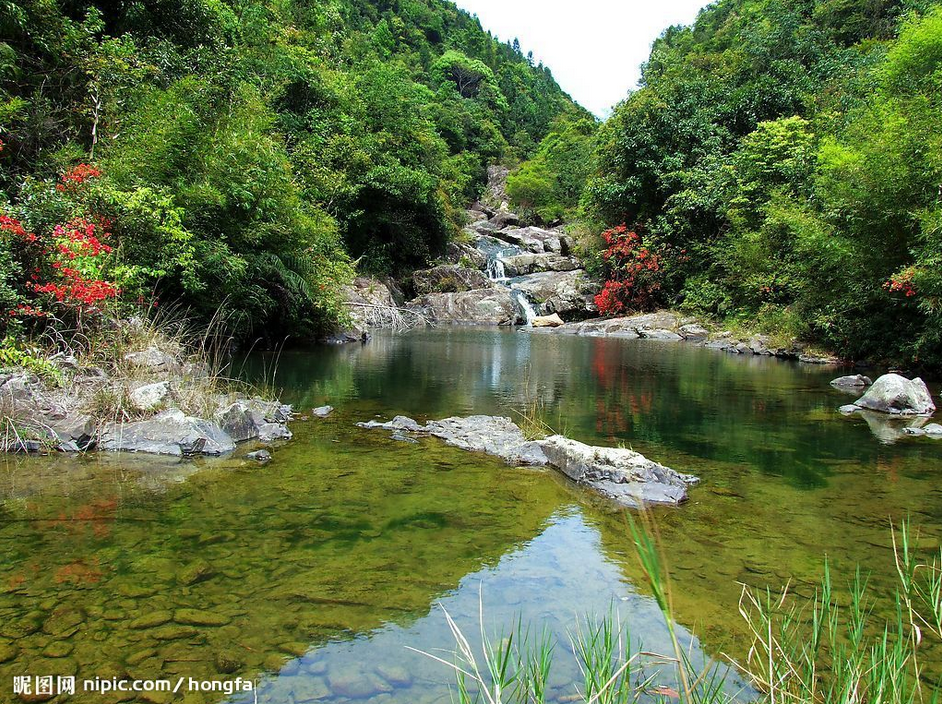
\includegraphics[width=0.7\linewidth]{zoomandshrinkor.png} 
 \end{figure}
\end{frame}

\begin{frame}
\frametitle{Zooming}
 \begin{figure}
 \caption{zoom}
 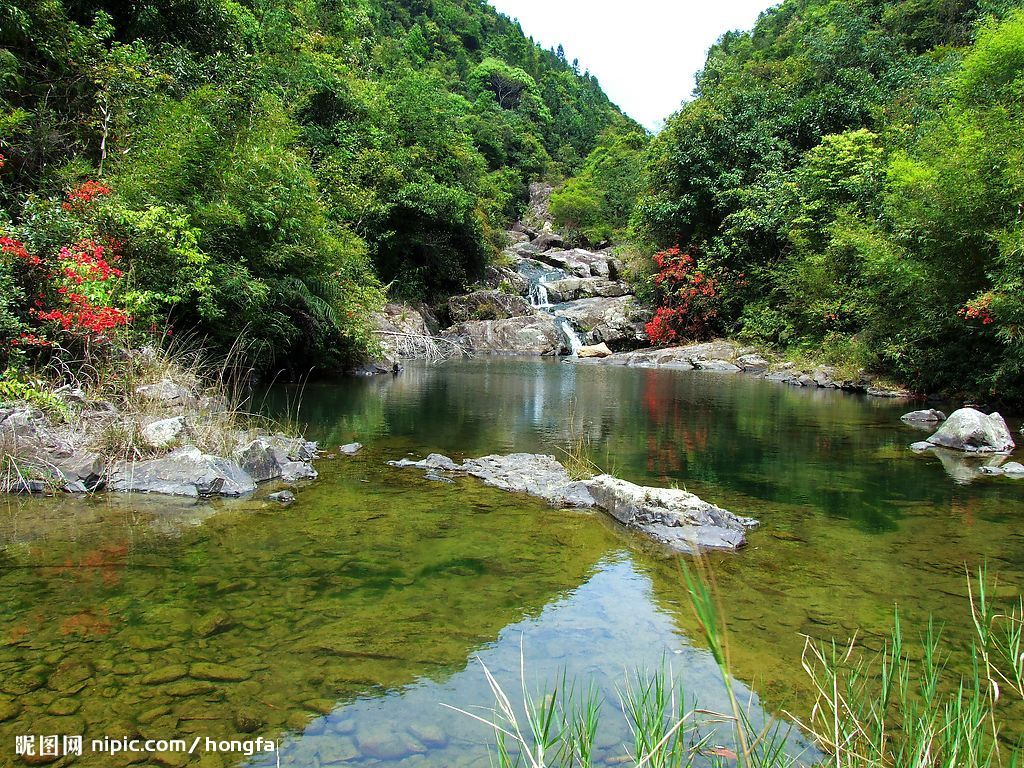
\includegraphics[width=0.7\linewidth]{fangda.png}
  \end{figure}

Nothing changed. 
\end{frame}


\begin{frame}
\frametitle{Shrinking}
 \begin{figure}
 \caption{shrink}
 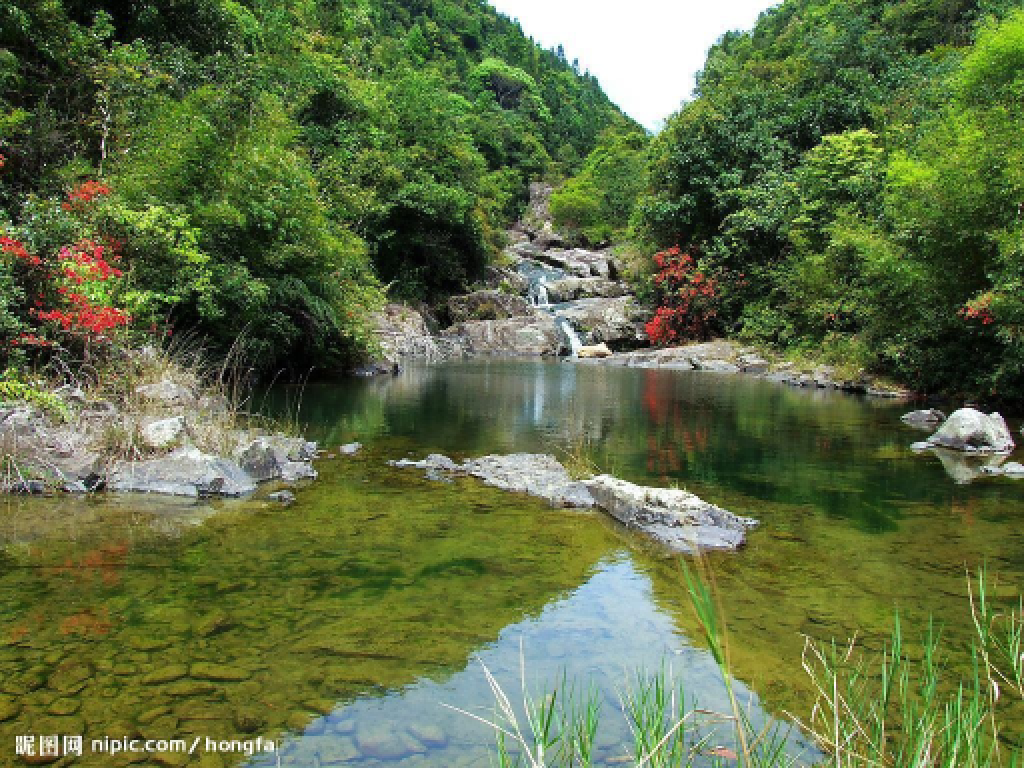
\includegraphics[width=0.7\linewidth]{suoxiao.png}
 \end{figure}
We could see the aliasing clearly.%可以看到混淆,为减小混淆,最好在缩小图像之前模糊一下图像。放大相当于过取样,之前不需要处理。
\end{frame}



%--------------------------------------------------------------------------
\subsection{2-D Discrete Fourier Transform and Its Inverse}%二维离散傅里叶变换及其反变换公式
\begin{frame}
\frametitle{2-D Discrete Fourier Transform and Its Inverse}
    
\begin{equation} \label{3}
F(u,v)=\sum_{x=0}^{M-1}\sum_{y=0}^{N-1}f(x,y)e^{-j2\pi(ux/M+vy/N)}
\end{equation}

where $f(x,y)$ is a dgital image of size $M*N$ . $u=0,1,2,\ldots,M-1$ and $v=0,1,2,\ldots,N-1$

The corresponding relationship between frequency domain and spatial domain.%公式即是频域与时域的对应关系

\begin{equation} \label{4}
f(x,y)=\frac{1}{MN}\sum_{u=0}^{M-1}\sum_{v=0}^{N-1}F(u,v)e^{j2\pi(ux/M+vy/N)}
\end{equation}

$x=0,1,2,\ldots,M-1$ and $y=0,1,2,\ldots,N-1$

\end{frame}

%-------------------------------------------------------------------------

\subsection{Properties of the 2-D Discrete Fourier Transform}%二维离散傅里叶变换的性质,后面会用到

\begin{frame}
\frametitle{Properties of the 2-D Discrete Fourier Transform}
    
\begin{itemize}
 \item Relationships Between Spatial and Frequency Intervals%%空间的频率间隔的关系
%%令 ∆T 和 ∆Z 表示样本间的间隔,相应离散频域变量间的间隔由
\begin{equation} \label{5}
\Delta u=\frac{1}{M\Delta T}
\end{equation}
\begin{equation} \label{6}
\Delta v=\frac{1}{N\Delta Z}
\end{equation} 
%给出
 \item Translation and Rotation %平移和旋转,将对称中心平移会用到

\begin{equation} \label{7}
f(x,y)e^{j2\pi (u_{0}x/M+v_{0}y/N)}\Leftrightarrow F(u-u_{0},v-v_{0})
\end{equation}

\begin{equation} \label{8}
f(x-x_{0},y-y_{0})\Leftrightarrow F(u,v)e^{-j2\pi (x_{0}u/M+y_{0}v/N)}
\end{equation}

Rotating $f(x,y)$ by an angle $\theta_{0}$ rotates $F(u,v)$ by the same angle.Rotating $F(u,v)$ rotates $f(x,y)$ by the same angle.

%若$f(x,y)$旋转$\theta_{0}$角度,则$F(u,v)$也旋转相同角度。若$F(u,v)$ 旋转一个角度,$f(x,y)$ 也旋转相同角度。

\item Periodicity %周期性

\end{itemize}

\end{frame}

\begin{frame}

\frametitle{Properties of the 2-D Discrete Fourier Transform}
    
\begin{itemize}

\item Symmetry Properties %对称性,在数字图像处理中有什么用?

About the center point of a sequence.
%对称(反对称)指的是关于序列中点的对称(反对称)
\begin{equation} \label{9}
w_{e}(x,y)=w_{e}(M-x,N-y)
\end{equation}

\begin{equation} \label{10}
w_{o}(x,y)=-w_{o}(M-x,N-y)
\end{equation}
%离散函数为奇函数的唯一方法是其所有样本的和为零
\item Spectrum and Phase Angle %傅里叶谱和相角

%零频率项F(0,0)与灰度成正比,所以经常有图像经过低通滤波器后直流分量被滤掉,平均灰度为0.图像不同傅里叶谱相同,相角一定不同。

While the magnitude of the 2-D DFT is an array Whose components determine the intensities in the image,the corresponding phase carry much of the information about where discernable objects are located in the image.



%当二维DFT的幅度是一个阵列时,其分量决定了图像中的灰度,相应的相位携带较多关于图像中可辨别的物体定位的信息(还有决定形状特点和特性内容)。 
\end{itemize}
\end{frame}

\begin{frame}

\frametitle{Properties of the 2-D Discrete Fourier Transform}
    
\begin{itemize}
\item The 2-D Convolution Theorem %二维卷积定理

Append zeros to solve wraparound error problem.%添0来避免周期过近,相互干扰导致缠绕错误

$f(x,y)$ and $h(x,y)$ are two image arrays of sizes $A\times B$ and $C\times D$ %$f(x,y)$ 和 $h(x,y)$分别是大小为 $A\times B$ 和 $C\times D$像素的图像阵列

The resulting padded images are both of size $P\times Q$.Where $P\geq A+C-1$ and $Q\geq B+D-1$


\end{itemize}
\end{frame}

%---------------------------------------------------------------------------

\subsection{Fourier Transformed Image}%经傅里叶变换后的图像
 \begin{frame}
\frametitle{Fourier Transform Image}
\begin{figure}
 \centering
 \caption{Original image}
 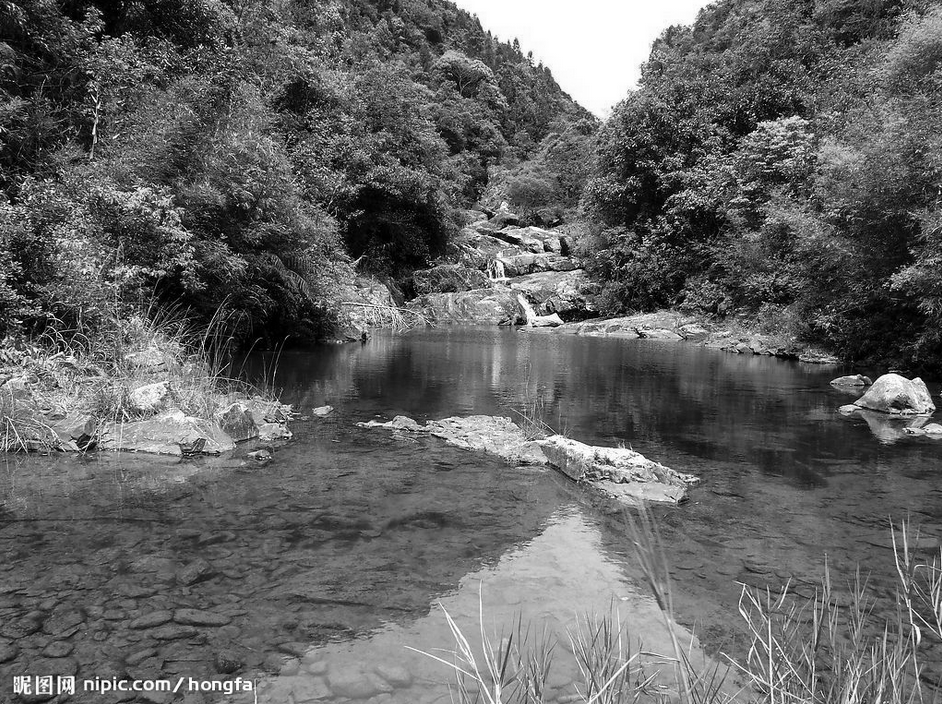
\includegraphics[width=0.8\linewidth]{orgn.png} 
 \end{figure}

 \end{frame}

\begin{frame}
\frametitle{Fourier Transform Image}
\begin{figure}
 \centering
 \caption{DFT image}
 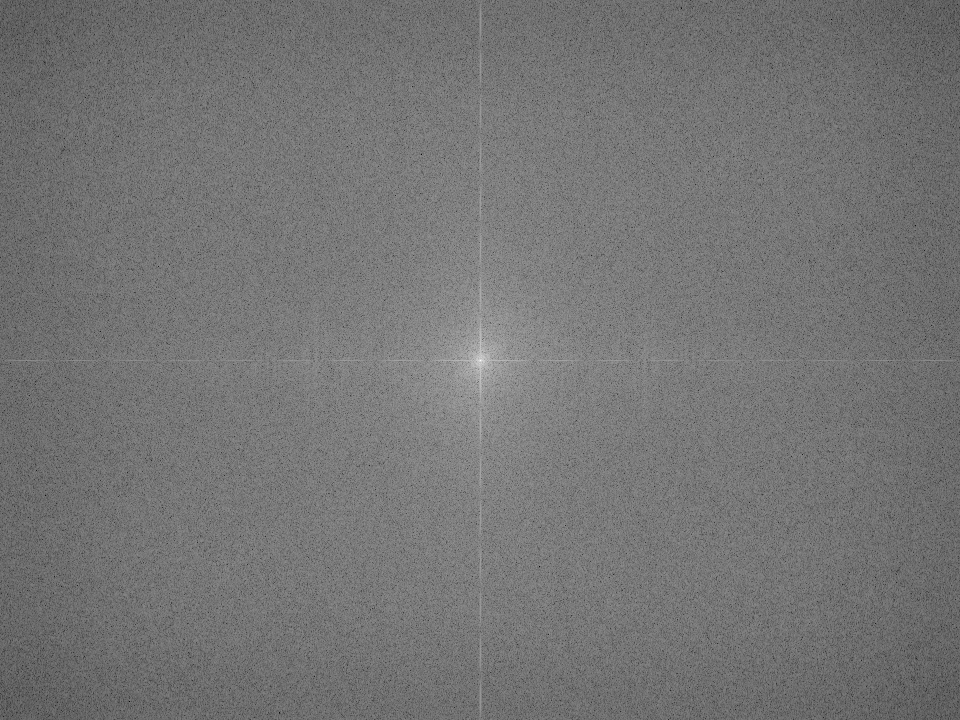
\includegraphics[width=0.8\linewidth]{magnitude.png} 
 \end{figure}
 \end{frame}

\begin{frame}
\frametitle{Rotating}
\begin{figure}
 \centering
 \caption{Original image}
 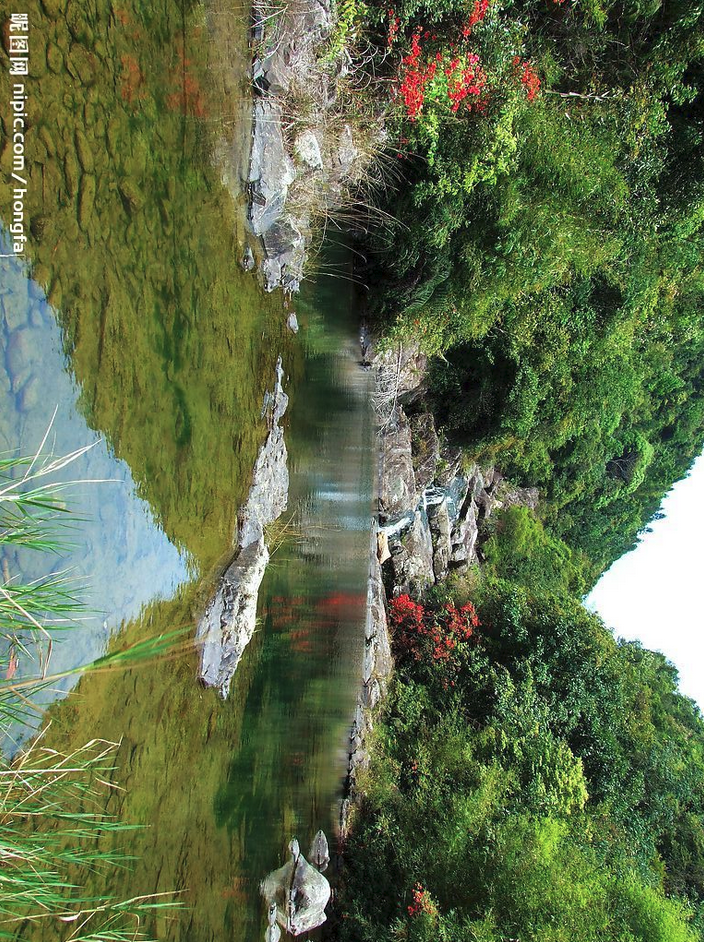
\includegraphics[width=0.5\linewidth]{rotateor.png} 
 \end{figure}
 \end{frame}

\begin{frame}
\frametitle{Rotating}
\begin{figure}
 \centering
 \caption{Rotating image}
 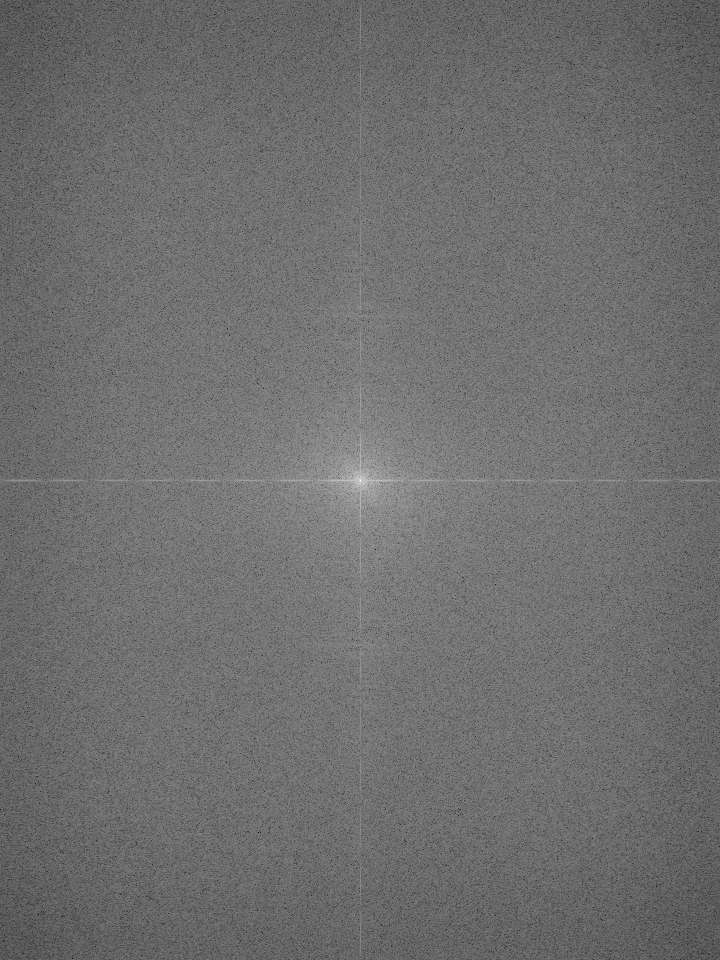
\includegraphics[width=0.5\linewidth]{rotate.png} 
 \end{figure}
 \end{frame}


\begin{frame}
\frametitle{Summary of Fourier Transform}
\begin{itemize}
\item The DFT of an image will be a frequency spectrum,whose magnitude is connected with its light and the phase is connected with its location about the original position.The spectrum rotates by the same angle of a rotated image.

\item The low frequencies correspond to the slowly varying intensity components of an image while the high frequencies correspond to faster intensity changes. 

%图像经过傅里叶变换会产生频谱图,幅值表现为对应点的亮度,相位表示相对于原始位置的偏移量。原图形旋转傅里叶也会跟着旋转相同角度。高频代表细节部分,高频部分越亮(幅值越大)代表细节部分越明显。低频代表变化缓慢的部分,低频部分越亮(幅值越大)代表变化缓慢的部分所占的比例较多。提取边缘的时候是不是就是先把低频滤掉?
\end{itemize}
 \end{frame}
%=======================================================================

\section{The Basic of Filtering in the Frequency Domain} %频域滤波基础

\subsection{Basic}
\begin{frame}
\frametitle{Basic}

Modifying the the Fourier transform to achieve a specific object,computing the inverse DFT to get back to the image domain.
%修改傅里叶变换以达到特殊目的,计算IDFT返回到图像域。

Equations:
   \begin{equation}    \label{11} %????
    g(x,y)=\mathscr{F}^{-1}[H(u,v)F(u,v)]
   \end{equation}

 \end{frame}

\subsection{Steps for Filtering}%频域滤波步骤

\begin{frame}
\frametitle{Steps for Filtering}%直方图均衡

\begin{enumerate}

\item An input image $f(x,y)$ of size $M\times N$,obtain the padding parameters  $P=2M$,$Q=2N$.
%大小为$M\times N$的输入图像$f(x,y)$,得到填充参数$P$ 和 $Q$,通常$P=2M$,$Q=2N$  
\item Form $f_{p}(x,y)$ of size $P\times Q$ by appending zeros to $f(x,y)$
%对$f(x,y)$添加0形成大小为$P\times Q$的填充后图像$f_{p}(x,y)$
\item Multiply $f_{p}(x,y)$ by $(-1)^{x+y}$ to center its transform
%用 $(-1)^{x+y}$乘以$f_{x,y}$移到其变换的中心
\item Compute the DFT from step 3

\item Generate a real,symmetric filter function,$H(u,v)$ of size $P\times Q$ with center at coordinates$(P/2,Q/2)$.$G(u,v)=H(u,v)F(u,v)$
%生成实的、对称的滤波函数$H(u,v)$,大小为$P\times Q$,中心在$(P/2,Q/2)$。$G(u,v)=H(u,v)F(u,v)$

\item $g_{p}(x,y)={real[\mathscr{F}^{-1}[G(u,v)]]}(-1)^{x+y}$, the real part is selected in order to ignore parasitic complex components resulting from computational inaccuracies.
%为忽略由于计算不准确导致的寄生复分量,选择了实部。
\item Obtain the final processed result,$g(x,y)$,by extracting the $M\times N$ region from the top,left quadrant of $g_{p}(x,y)$ 
%从$g_{p}(x,y)$ 的左上限提取$M\times N$区域,得到最终处理结果$g(x,y)$

\end{enumerate}

\end{frame}
%=======================================================================

\section{Filters}%滤波器

\subsection{Lowpass Filters}

\begin{frame}
\frametitle{Lowpass Filters}
Image smoothing.%平滑(模糊)图像
\begin{figure}
 \centering
 \caption{Origin image}
 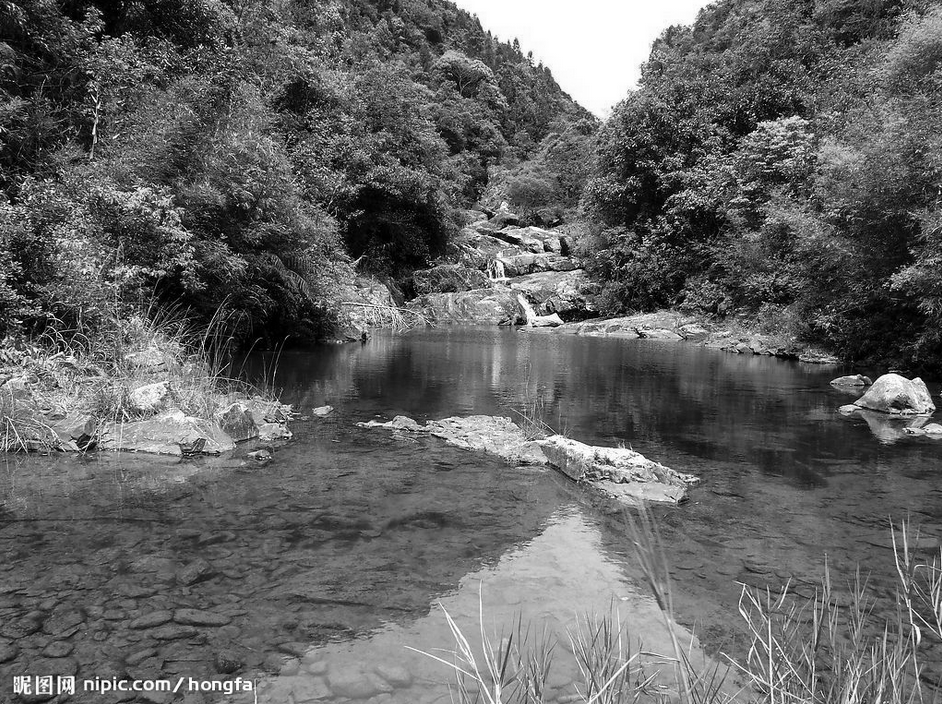
\includegraphics[width=0.8\linewidth]{orgn.png} 
 \end{figure}
 \end{frame}

\begin{frame}
\frametitle{Ideal Lowpass Filters}
\begin{figure}
 \centering
 \caption{ILPF image $D_{0}=100$}
 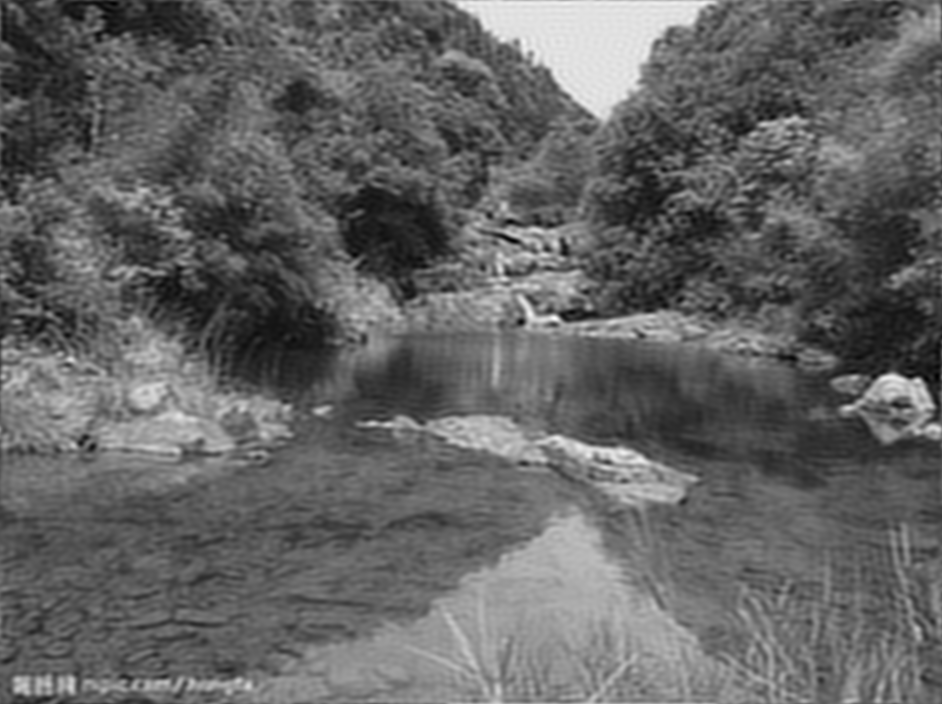
\includegraphics[width=0.8\linewidth]{ilpf.png} 
 \end{figure}
\end{frame}


\begin{frame}
\frametitle{Butterworth Lowpass FIlters}
\begin{figure}
 \centering
 \caption{BLPF image $D_{0}=100,n=2$}
 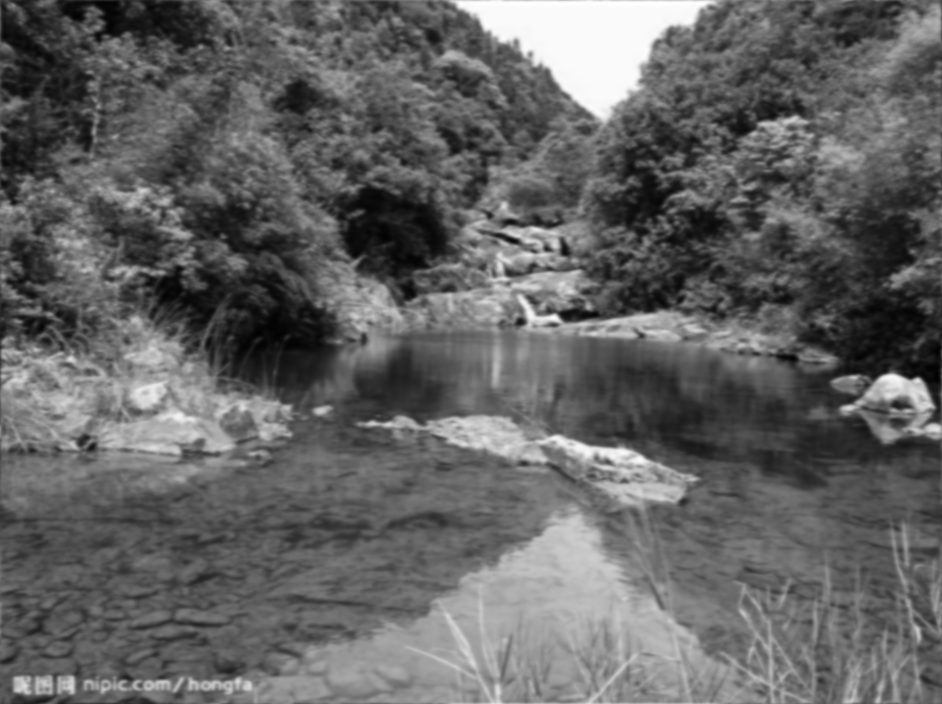
\includegraphics[width=0.8\linewidth]{blpf.png} 
 \end{figure}
\end{frame}

\begin{frame}
\frametitle{Gaussian Lowpass FIlters}
\begin{figure}
 \centering
 \caption{GLPF image $D_{0}=100$}
 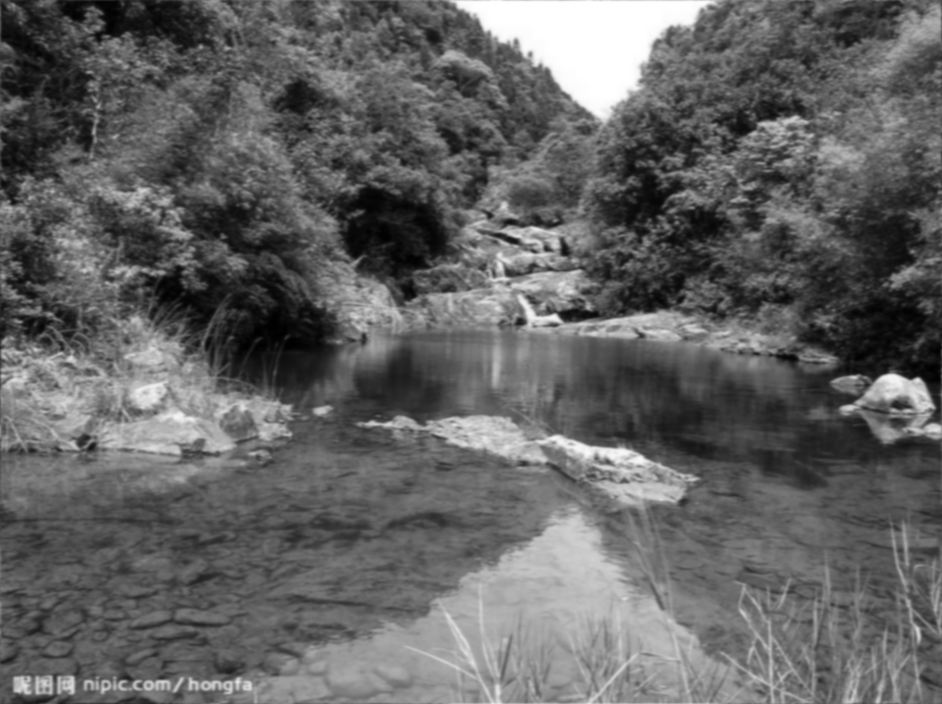
\includegraphics[width=0.8\linewidth]{glpf.png} 
 \end{figure}
\end{frame}

\begin{frame}
\frametitle{FIlters Summery}
ILPF:ringing.%有振铃

BLPF:good compromise between effective lowpass filtering and acceptable ringing.%在可接受的低通滤波和振铃之间由很好的折中

GLPF:no ringing,less smoothing than the BLPF.%无振铃,平滑结果稍差
\end{frame}
%------------------------------------------------------------------------


\subsection{Highpass Filters}


\begin{frame}
\frametitle{Highpass Filters-Butterworth Highpass Filters}
\begin{figure}
 \centering
 \caption{BHPF image}
 
\includegraphics[width=0.8\linewidth]{bhpf1.png} 
 \end{figure}
 \end{frame}

\begin{frame}
\frametitle{Highpass Filters}
Image Sharpening.%锐化图像

\begin{figure}
 \centering
 \caption{Origin image}
 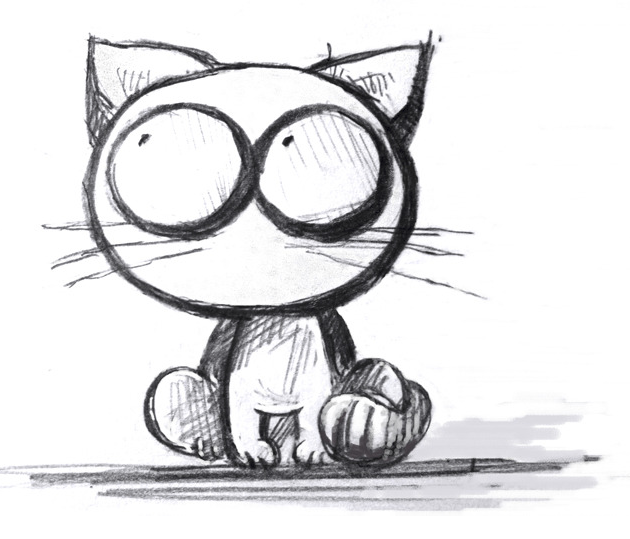
\includegraphics[width=0.8\linewidth]{horgn.png} 
 \end{figure}
 \end{frame}

\begin{frame}
\frametitle{Ideal Highpass Filters}
\begin{figure}
 \centering
 \caption{IHPF image}
 
\includegraphics[width=0.8\linewidth]{ihpf.png} 
 \end{figure}
 \end{frame}

\begin{frame}
\frametitle{Butterworth Highpass Filters}
\begin{figure}
 \centering
 \caption{BHPF image}
 
\includegraphics[width=0.8\linewidth]{bhpf.png} 
 \end{figure}
 \end{frame}


\begin{frame}
\frametitle{Equalization}
\begin{figure}
 \centering
 \caption{Equal image}
 
\includegraphics[width=0.8\linewidth]{equa1.png} 
 \end{figure}
 \end{frame}

\begin{frame}
\frametitle{Gaussian Highpass Filters}
\begin{figure}
 \centering
 \caption{GHPF image}
 
\includegraphics[width=0.8\linewidth]{ghpf.png} 
 \end{figure}
 \end{frame}

\begin{frame}
\frametitle{High-Frequency-Emphasis Filters}%高频强调滤波
\begin{equation} \label{12}
g(x,y)=\mathscr{F}^{-1}\{[k_{1}+k_{2}*H_{HP}(u,v)]F(u,v)\}
\end{equation}

 \qquad   $k_{1}\geq 0$ gives controls of the offset from the origin
%给出了控制距原点的偏移量,k2<1时类似于模糊
\end{frame}

\begin{frame}
\frametitle{High-Frequency-Emphasis Filters}
\begin{figure}
 \centering
 \caption{$k_{1}=1,k_{2}=4$}
 
\includegraphics[width=0.8\linewidth]{k4hfef1.png} 
 \end{figure}
 \end{frame}

\begin{frame}
\frametitle{High-Frequency-Emphasis Filters}
\begin{figure}
 \centering
 \caption{$k_{1}=1,k_{2}=4$}
 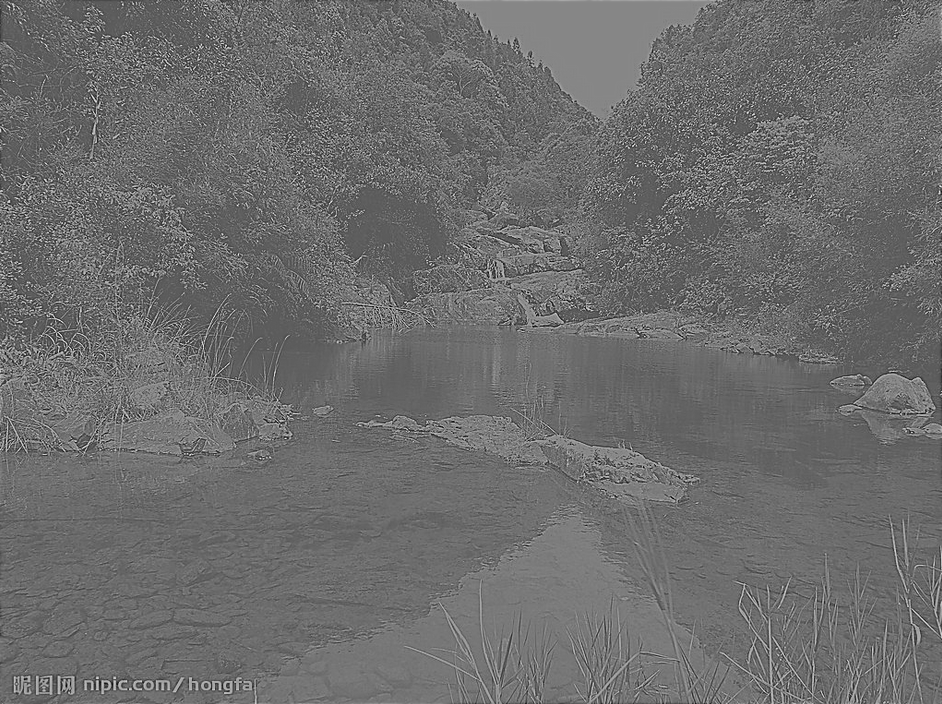
\includegraphics[width=0.8\linewidth]{k4hfef2.png} 
 \end{figure}
 \end{frame}

\begin{frame}
\frametitle{Homomorphic Filters}%同态滤波
\begin{figure}
 \centering
 \caption{Homo image}
 
\includegraphics[width=0.5\linewidth]{homo.png} 
 \end{figure}
A procedure for improving the appearance of an image by simultaneous intensity range compres-sion(ln) and contrast enhancement(filter).
%通过同时压缩灰度范围(ln)和增强对比度(filter)来改善一副图像的表现,与高频强调滤波器类似
 \end{frame}

\subsection{Selective Filters}%选择性滤波

\begin{frame}
\frametitle{Selective Filters}
\begin{figure}
 \centering
 \caption{Origin image}
 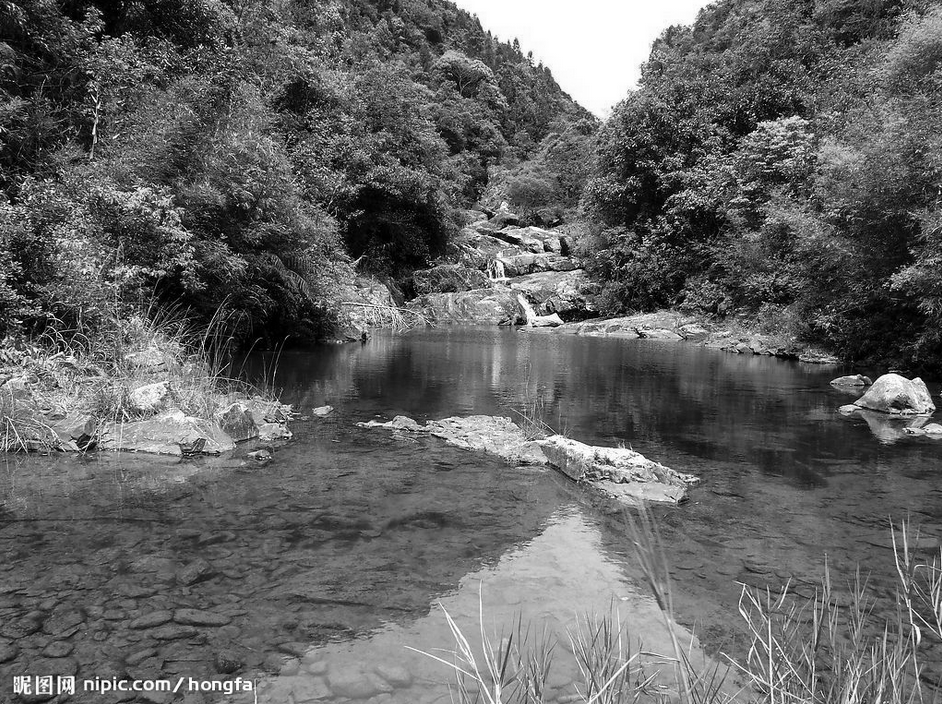
\includegraphics[width=0.8\linewidth]{orgn.png} 
 \end{figure}
\end{frame}

\begin{frame}
\frametitle{Bandpass Filters}%带通滤波
\begin{figure}
 \centering
 \caption{$D_{0}=100,w=40$}%截止频率为100,带宽为40,像高通滤波
 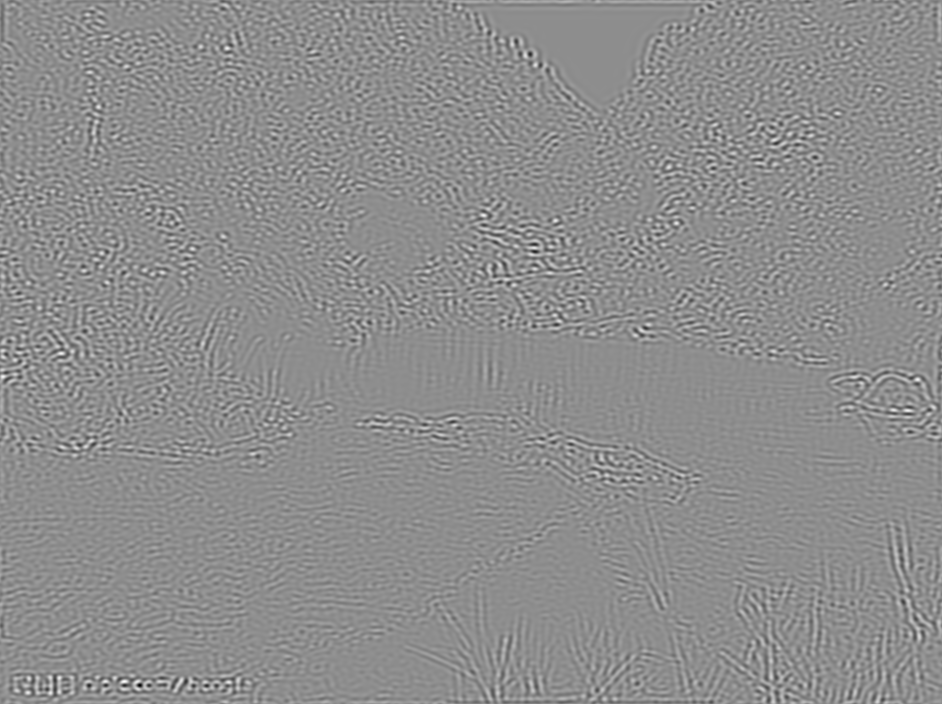
\includegraphics[width=0.8\linewidth]{w40bandpass.png} 
 \end{figure}
\end{frame}

\begin{frame}
\frametitle{Bandpass Filters}%带通滤波
\begin{figure}
 \centering
 \caption{$D_{0}=100,w=80$}%截止频率为100,带宽为80
 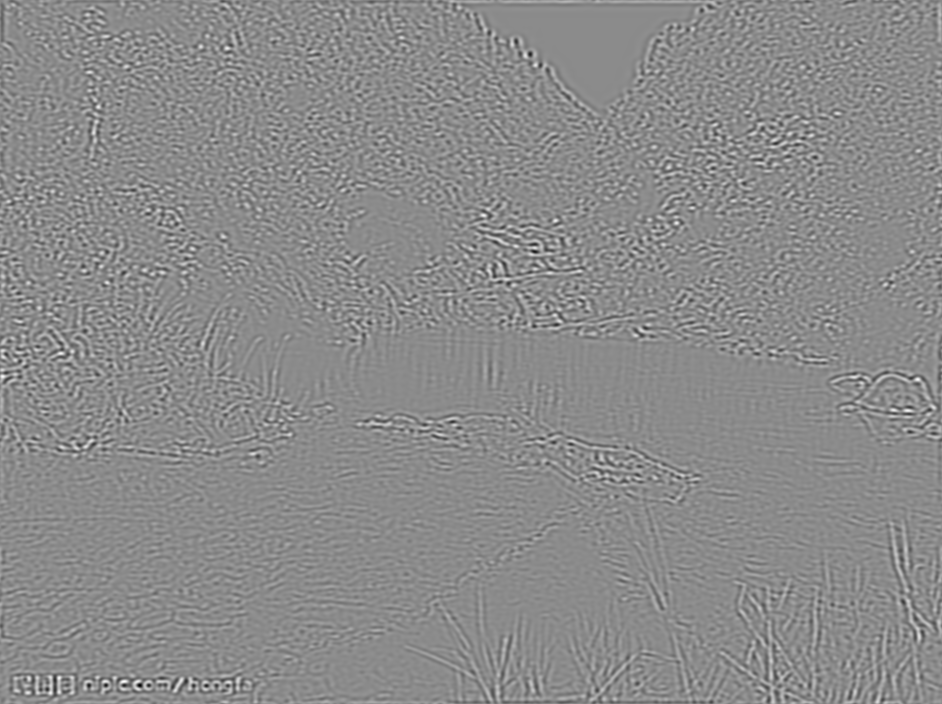
\includegraphics[width=0.8\linewidth]{w80bandpass.png} 
 \end{figure}
\end{frame}

\begin{frame}
\frametitle{Bandpass Filters}%带通滤波
\begin{figure}
 \centering
 \caption{$D_{0}=5,w=140$}%截止频率为100,带宽为80,像低通滤波
 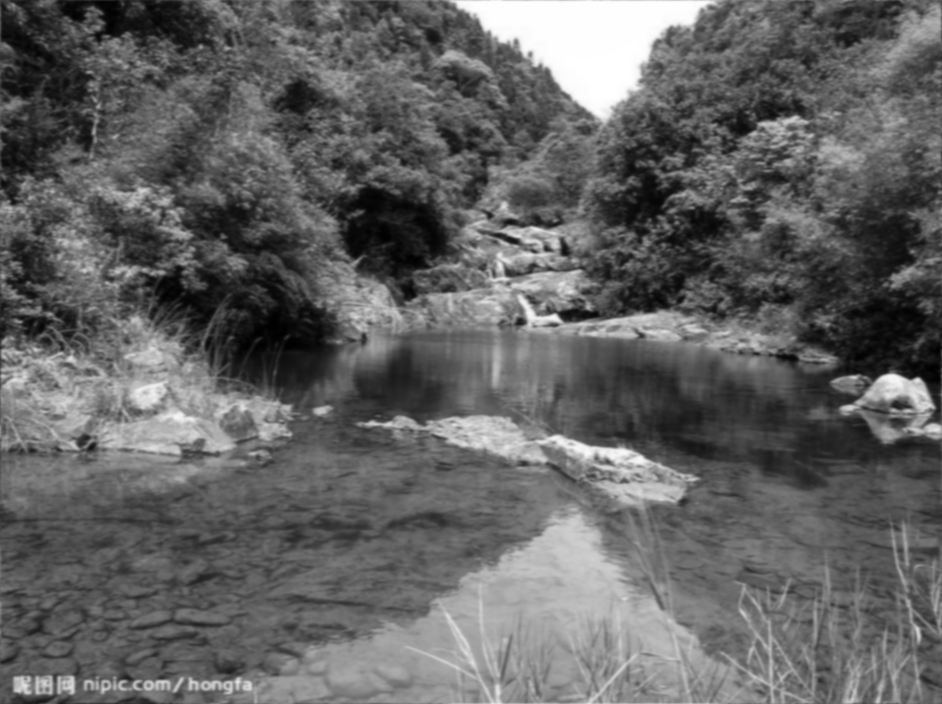
\includegraphics[width=0.8\linewidth]{d05w140bandpass.png} 
 \end{figure}
\end{frame}
%类似于局部直方图处理

\begin{comment}
\end{comment}
%两个补0,卷积(以及傅里叶变换相乘时,包括滤波时的傅里叶变换相乘),方便快速对函数进行傅里叶变换(opencv上介绍)
%=======================================================================

\end{document}
